\documentclass[12pt,a4paper]{article}

\usepackage[margin=1in]{geometry}
\usepackage{graphicx}
\usepackage{booktabs}
\usepackage{hyperref}

\title{Student Performance Analytics and Prediction System}
\author{Project Team}
\date{\today}

\begin{document}

\maketitle

\section{Introduction}
This project analyzes student academic performance using
Python, data analysis, visualization, and machine learning.

\section{Objectives}
\begin{itemize}
    \item Analyze student marks and attendance.
    \item Calculate subject-wise average marks.
    \item Visualize the distribution of student performance.
    \item Estimate average marks using previous scores and attendance.
    \item Test the correctness of the program.
\end{itemize}

\section{Dataset}
The dataset contains student IDs, marks in Mathematics,
Physics and Programming, attendance, and previous scores.

\section{Methodology}
The system validates the dataset, calculates descriptive
statistics, creates visualizations, and trains a
linear regression model.

\section{Results}

\subsection{Average Marks by Subject}

The bar chart compares the average marks obtained
in Mathematics, Physics, and Programming.

\begin{figure}[htbp]
    \centering
    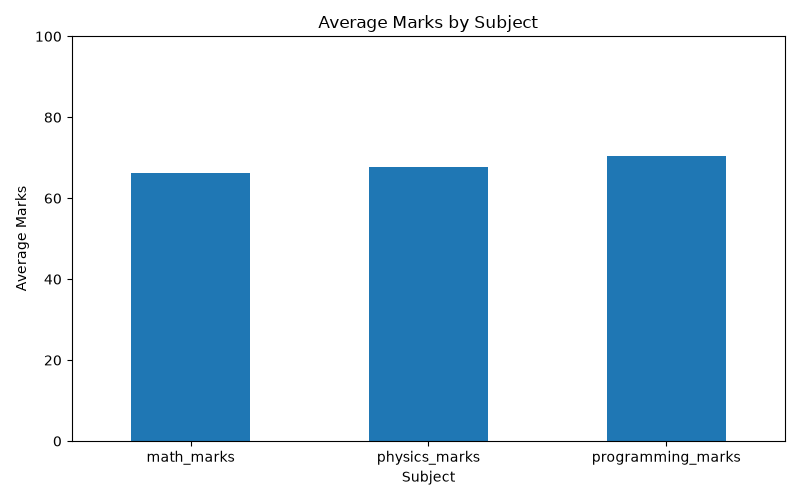
\includegraphics[width=0.85\textwidth]
    {subject_averages.png}
    \caption{Average marks by subject}
    \label{fig:subject-averages}
\end{figure}

\subsection{Distribution of Student Average Marks}

The histogram illustrates how student average marks
are distributed across different score ranges.

\begin{figure}[htbp]
    \centering
    \includegraphics[width=0.85\textwidth]
    {average_distribution.png}
    \caption{Distribution of student average marks}
    \label{fig:average-distribution}
    
\end{figure}

\subsection{Prediction Model Evaluation}

The Linear Regression model was evaluated using
Mean Absolute Error (MAE). The model reported an MAE
of 1.61 marks on the evaluation data.

\subsection{Example Student Prediction}

The model was provided with a previous score of 70
and an attendance percentage of 85\%. It estimated
the student's average marks to be 69.06 out of 100.

This prediction is an estimate and should not be
considered a guaranteed academic result.

\subsection{Subject-Wise Analysis}

The dataset was analyzed to calculate the average
marks in Mathematics, Physics, and Programming.
The subject-wise averages, class pass percentage,
and graphs will be included after the analysis
results have been recorded.

\section{Conclusion}
The project demonstrates how Python can be used to
analyze and visualize student performance. Predictions
are estimates and depend on the quality of the dataset.

\end{document}